\chapter{\ifproject%
\ifenglish Experimentation and Results\else การทดลองและผลลัพธ์\fi
\else%
\ifenglish System Evaluation\else การประเมินระบบ\fi
\fi}

ในบทนี้จะทดสอบเกี่ยวกับการทํางานในฟังก์ชันหลักๆ ของแอปพลิเคชัน โดยเนื้อหาจะกล่าวถึงคือโมดูลการทํางานต่างๆ ของระบบ

\subsection{การทดสอบระบบ API ของ backend}
เนื่องจาก API หลักๆในระบบ จะถูกส่งด้วย GraphQL เราจึงได้มีการทดสอบ ทุก Resolvers ในระบบ เเละจากการทดสอบไม่พบข้อผิดพลาดใดๆ
\begin{center}
    \begin{minipage}[c]{0.5\linewidth}
       \begin{itemize}
         \item ยกตัวอย่างการดึงข้อมูลหมวดต่างๆ ที่เก็บรายวิชา
       \end{itemize}
    \end{minipage}
  \end{center}

  \begin{figure}[H]
    \begin{center}
      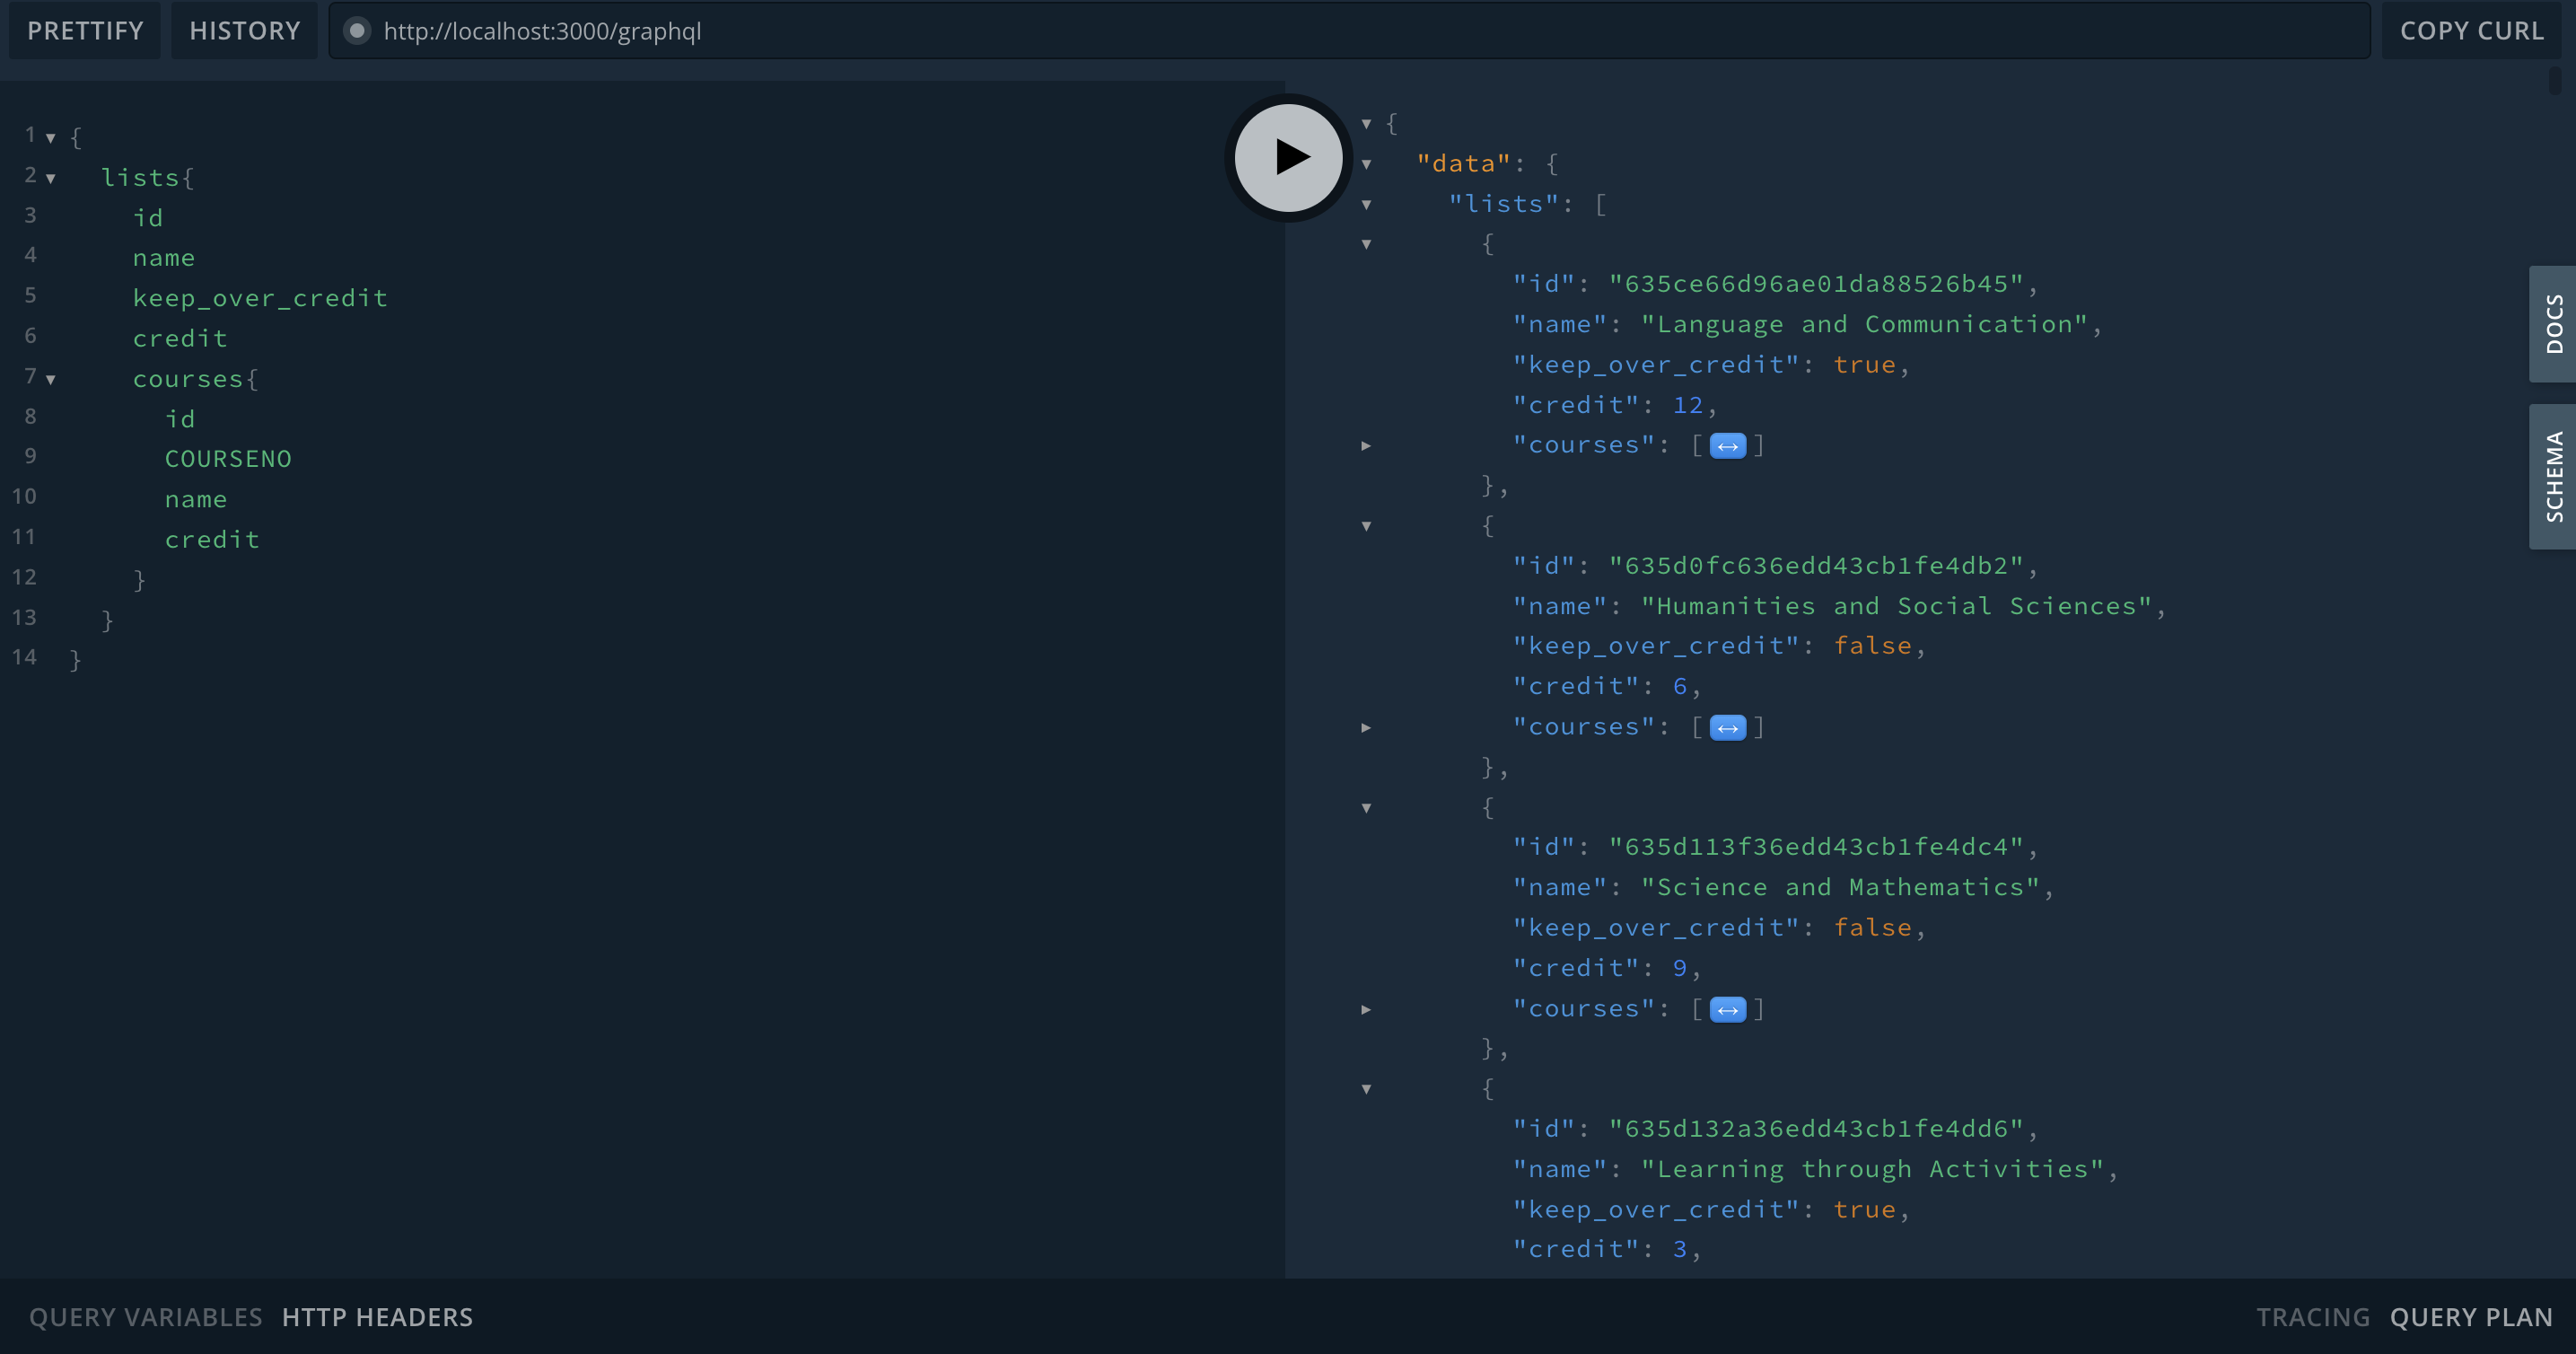
\includegraphics[width=0.8\textwidth]{gql.png}
      \caption{lists data}
      \label{fig:gql}
    \end{center}
  \end{figure}
    
\subsection{ผลตอบรับและความคิดเห็นของผู้ใช้งาน}
หลังจากการพัฒนาระบบแสดงความคืบหน้าในการสำเร็จการศึกษา 
ทางผู้พัฒนาได้ปล่อยเวอร์ชันทดลองใช้งานให้กับนักศึกษาและอาจารย์ในภาควิชาคอมพิวเตอร์และภาควิชาเทคโนโลยีสารสนเทศพร้อมทั้งแนบแบบสอบถาม
เพื่อเก็บความพึงพอใจต่อภาพรวม UX/UI และ flow ของระบบ โดยมีนักศึกษาที่เข้ามาทดลองใช้งานระบบรวม 11 คน 
(นับจำนวนจากข้อมูลใน database ที่มีการ login เข้ามาในระบบ) แต่กลับพบว่ามีนักศึกษาเพียง 6 คนเท่านั้นที่ทำการตอบแบบสอบถาม 
พบว่าผลตอบลัพธ์และความคิดเห็นของผู้ใช้งานที่มีต่อเว็บแอปพลิเคชันมีแนวโน้มที่ดี ซึ่งสามารถสรุปผลตอบลัพธ์ได้ดังรูปที่ 1 และ รูปที่ 2 
ซึ่งเป็นความพีงพอใจต่อการใช้งานและภาพรวมของเว็บแอปพลิเคชัน

\begin{figure}[H]
    \begin{center}
      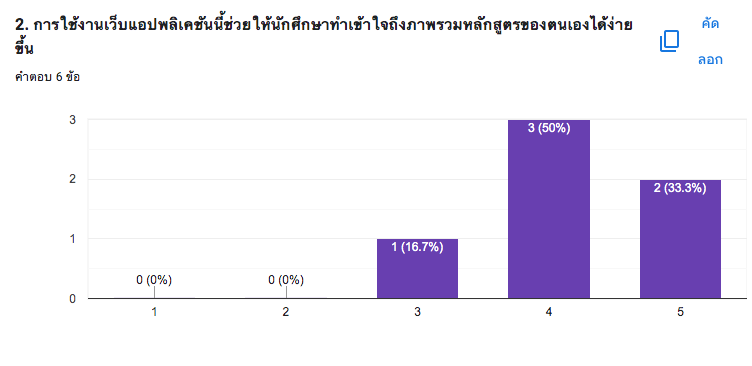
\includegraphics[width=0.8\textwidth]{toon1.png}
      \caption{ความพีงพอใจต่อการใช้งานและภาพรวมของเว็บแอปพลิเคชัน}
      \label{fig:toon1}
    \end{center}
\end{figure}

\begin{figure}[H]
    \begin{center}
      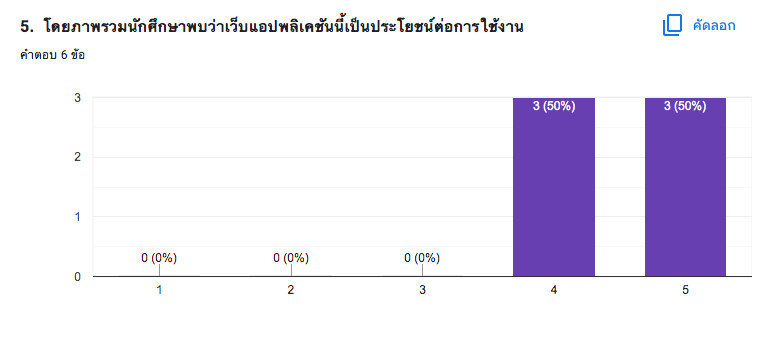
\includegraphics[width=0.8\textwidth]{toon2.png}
      \caption{ความพีงพอใจต่อภาพรวมของเว็บแอปพลิเคชัน}
      \label{fig:toon2}
    \end{center}
\end{figure}
    